%%%%%%%%%%%%%%%%%%%%%%%%%%%%%%%%%%%%%%%%%
% University/School Laboratory Report
% LaTeX Template
% Version 3.0 (4/2/13)
%
% This template has been downloaded from:
% http://www.LaTeXTemplates.com
%
% Original author:
% Linux and Unix Users Group at Virginia Tech Wiki 
% (https://vtluug.org/wiki/Example_LaTeX_chem_lab_report)
%
% License:
% CC BY-NC-SA 3.0 (http://creativecommons.org/licenses/by-nc-sa/3.0/)
%
%%%%%%%%%%%%%%%%%%%%%%%%%%%%%%%%%%%%%%%%%

%----------------------------------------------------------------------------------------
%	PACKAGES AND DOCUMENT CONFIGURATIONS
%----------------------------------------------------------------------------------------

\documentclass{article}

\usepackage[version=3]{mhchem} % Package for chemical equation typesetting
\usepackage{siunitx} % Provides the \SI{}{} command for typesetting SI units

\usepackage{graphicx}
\usepackage{caption}
\usepackage{subcaption}
\usepackage{cancel}

\usepackage{float}

\usepackage[T1]{fontenc} % allow small bold caps

\usepackage{listings}
\usepackage{color}

\definecolor{dkgreen}{rgb}{0,0.6,0}
\definecolor{gray}{rgb}{0.5,0.5,0.5}
\definecolor{mauve}{rgb}{0.58,0,0.82}

\lstset{frame=tb,
  language=Matlab,
  aboveskip=2mm,
  belowskip=2mm,
  showstringspaces=false,
  columns=flexible,
  basicstyle={\small\ttfamily},
  numbers=none,
  numberstyle=\tiny\color{gray},
  keywordstyle=\color{blue},
  commentstyle=\color{dkgreen},
  stringstyle=\color{mauve},
  breaklines=true,
  breakatwhitespace=true
  tabsize=2
}

\setlength\parindent{0pt} % Removes all indentation from paragraphs

\renewcommand{\labelenumi}{\alph{enumi}.} % Make numbering in the enumerate environment by letter rather than number (e.g. section 6)

\usepackage[margin=1in]{geometry}

\usepackage{amssymb}


%\usepackage{times} % Uncomment to use the Times New Roman font

%----------------------------------------------------------------------------------------
%	Title
%----------------------------------------------------------------------------------------

\begin{document}
\pagenumbering{gobble}

\title{6.s02: EECS II - From A Medical Perspective}
\author{
  Ryan Lacey <rlacey@mit.edu>\\
  \footnotesize \texttt{Collaborator(s): Jorge Perez}
}
        
\maketitle
        


\begin{enumerate}
\item[1.]
	\begin{enumerate}
	\item[(a)]
		The fundamental period of this DT signal is $N=7$. Let $\Omega_0 = \dfrac{2\pi}{7}$\\
		
		Evaluating the synthesis equation for the period of $X[k]$ between $k=-3$ and $k=3$\\
		
		$x[n] = \dfrac{1}{2}\left(e^{j2\Omega_{0}n} + e^{-j2\Omega_{0}n}\right)$\\
		
		$x[n] = \cos\left(2\Omega_{0}n\right) = \cos\left(\frac{4\pi}{7}n\right)$

\bigskip

	\item[(b)]
		$x[n] = \cos\left(\Omega n\right)$\\
		
		$\omega = \dfrac{\Omega}{T_{s}} = \dfrac{\frac{4\pi}{7}}{0.1} = \dfrac{40\pi}{7}$\\
		
		$x[t] = \cos\left(\omega t\right) = \cos\left(\dfrac{40\pi}{7} t\right) $

\bigskip

	\item[(c)]
		The fundamental period of this DT signal is $N=7$. Let $\Omega_0 = \dfrac{2\pi}{7}$\\
		
		Evaluating the synthesis equation for the period of $X[k]$ between $k=-3$ and $k=3$\\
		
		$x[n] = \dfrac{1}{2}\left(e^{j3\Omega_{0}n} + e^{-j3\Omega_{0}n}\right)$\\
		
		$x[n] = \cos\left(3\Omega_{0}n\right) = \cos\left(\frac{6\pi}{7}n\right)$

\bigskip

	\item[(d)]
		$x[n] = \cos\left(\Omega n\right)$\\
		
		$\omega = \dfrac{\Omega}{T_{s}} = \dfrac{\frac{6\pi}{7}}{0.15} = \dfrac{40\pi}{7}$\\
		
		$x[t] = \cos\left(\omega t\right) = \cos\left(\dfrac{40\pi}{7} t\right) $
	\end{enumerate}

\newpage

\item[2.]
	\begin{enumerate}
	\item[(a)]
		$H_d[k] = \dfrac{I[k]}{Q[k]}$\\
		
		We want to solve for $I[k]$\\
		
		$I[t] = Q[t] - Q[t-1] \implies I[k] = Q[k] \left(1 - e^{-j\Omega_0k}\right)$\\
		
		$\therefore H_d[k] = 1 - e^{-j\Omega_0k}$\\

\bigskip

	\item[(b)]
		$H_a[k] = \left(H_d[k]\right)^{-1}$\\
		
		$H_a[k] = \dfrac{1}{1 - e^{-j\Omega_0k}}$

\bigskip

	\item [(c)] $\:$ \\
		\begin{figure}[!htb]
		\minipage{\textwidth}
			  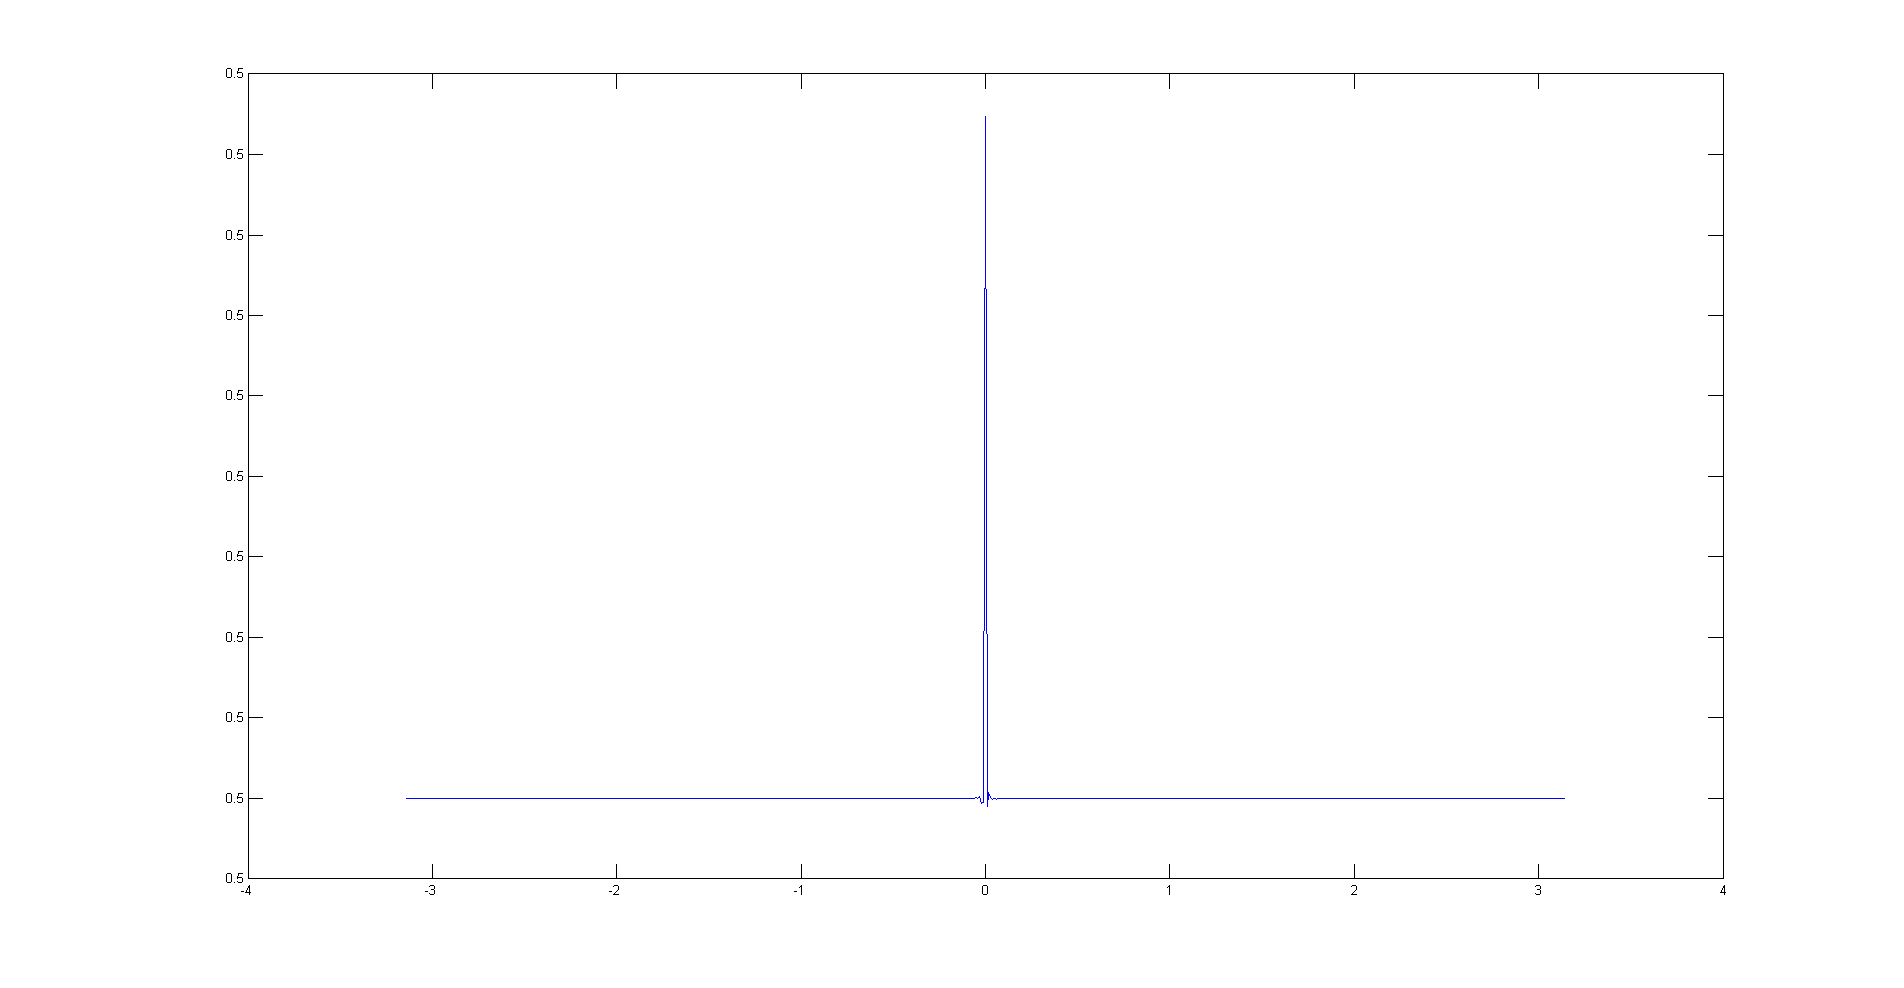
\includegraphics[width=\linewidth]{../images/Problem3Graph.png}
		  \caption{$H_a$ low-pass filter.}
		\endminipage\hfill
		\end{figure}

	\end{enumerate}

\newpage

\item[3.]
	\begin{enumerate}
	\item[(a)]
		$y\left[n\right] = \left(\displaystyle\sum_{i=1}^{3} \alpha^i\right)^{-1} \left(\alpha x[n] + \alpha^2 x[n-1] + \alpha^3 x[n-2]\right)$\\
		
		$y\left[n\right] = \left(1.952\right)^{-1} \left(0.8 x[n] + 0.64 x[n-1] + 0.512 x[n-2]\right)$

\bigskip

	\item[(b)]
		Adding in the appropriate coefficients from Lab 3's prelab yields\\
		
		$H\left[k\right] = \left(\dfrac{1}{3} \times \dfrac{1}{\sum_{i=1}^{3} \alpha^i}\right) \left(\alpha^1 + \alpha^2 e^{-jk\omega} + \alpha^3 e^{-2jk\omega}\right)$\\
		
		$H\left[k\right] = \left(0.171\right) \left(0.8 + 0.64 e^{-jk\omega} + 0.512 e^{-2jk\omega}\right)$
	\end{enumerate}

\newpage

\item[4.]
	\begin{enumerate}
	\item[(a)] $\:$ \\
		\begin{figure}[!htb]
		\minipage{\textwidth}
		  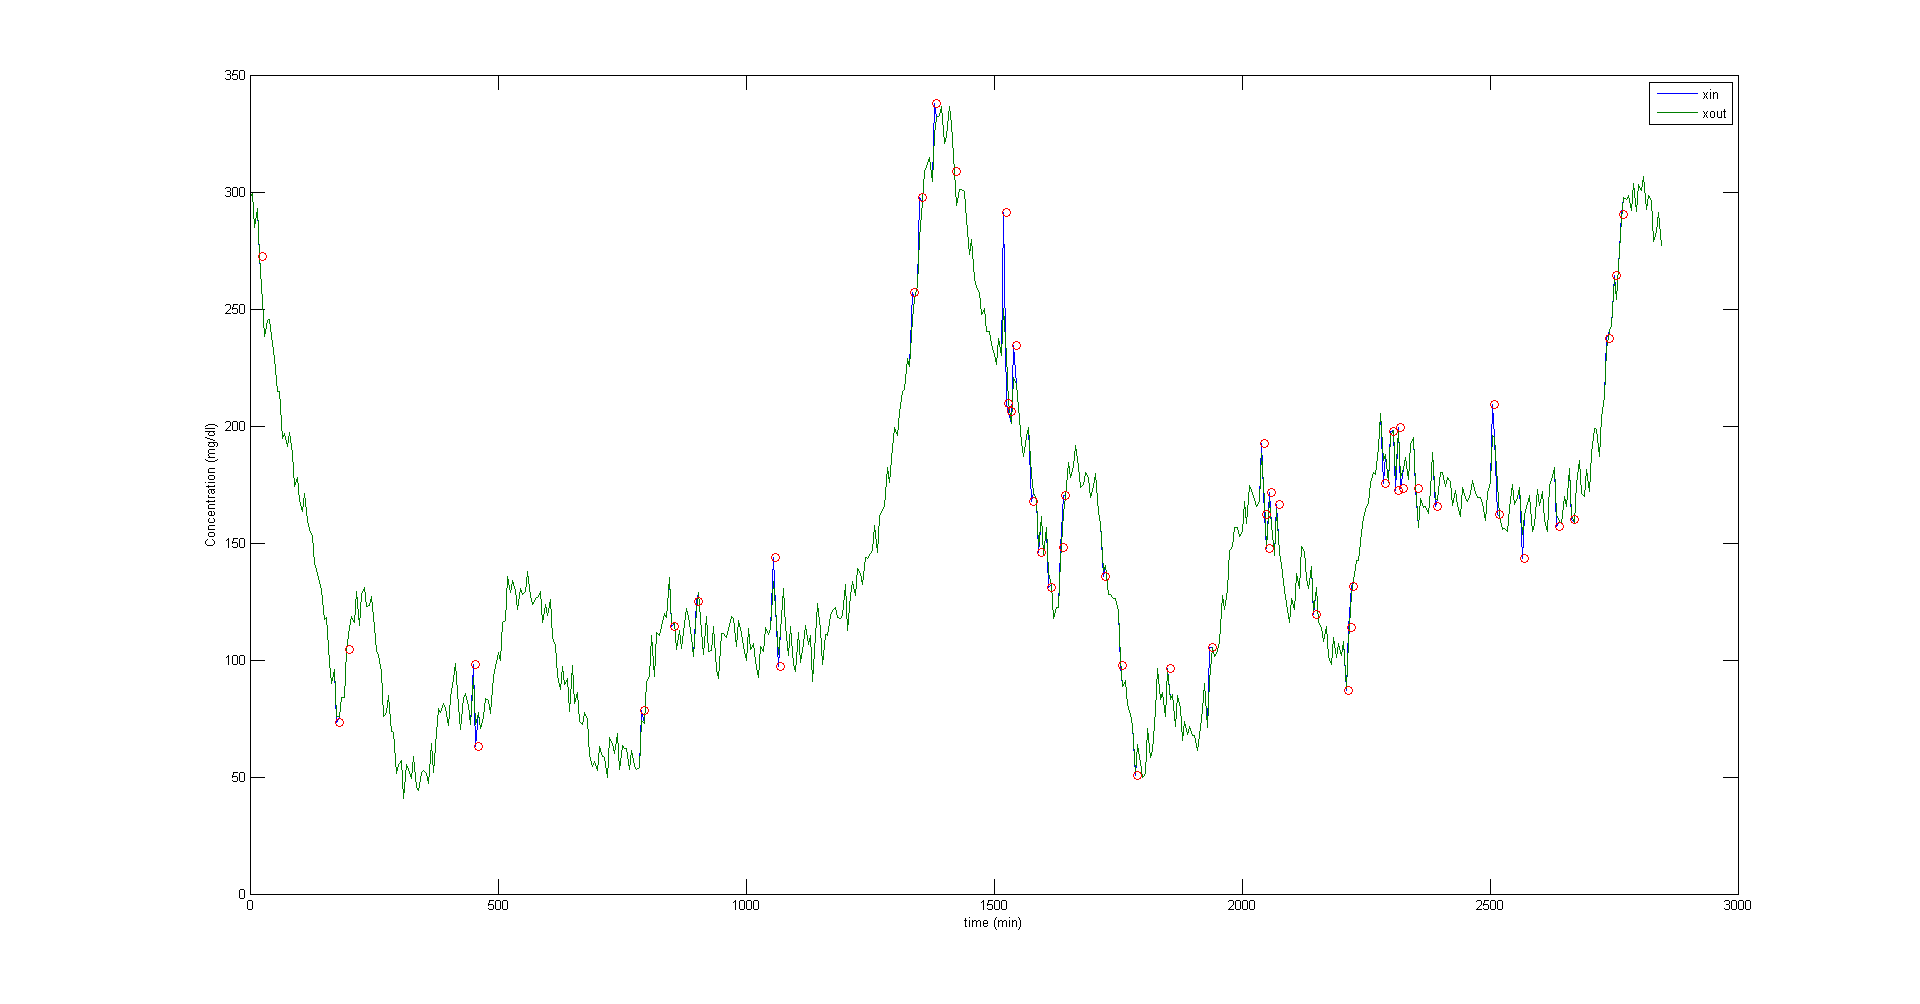
\includegraphics[width=\linewidth]{../images/Problem4Graph.png}
		  \caption{Continuous glucose monitor with overlay of signal with artifacts removed. Points where sensor input was altered is highlighted with red circles.}
		\endminipage\hfill
		\end{figure}

\bigskip 

\begin{lstlisting}   
function [xout, changes] = cgmprefilter(xin, t)
    len = length(t);
    xout = zeros(len, 1);
    changes = zeros(len, 1);
    xout(1) = xin(1);
    for i = 2:length(t)
        diff = xin(i) - xout(i-1);
        if (abs(diff) > 20)
            changes(i) = 1;
            if (diff > 0)
                xout(i) = xout(i-1) + 20;
            else
                xout(i) = xout(i-1) - 20;
            end
        else
            xout(i) = xin(i);
        end
    end
end
\end{lstlisting}

\bigskip 

	\item[(b)]
	Input data altered at 52 locations.
	\end{enumerate}

\end{enumerate}

\end{document}